\documentclass{article}
\usepackage{geometry}
\usepackage{amsmath}
\usepackage{titling}
\usepackage{graphicx}
\usepackage{hyperref}

\hypersetup{colorlinks=true,urlcolor=cyan,linkcolor=blue}

\pretitle{\begin{center}\huge}
\posttitle{\end{center}}
\preauthor{\begin{center}\small}
\postauthor{\end{center}}
\predate{\begin{center}\footnotesize}
\postdate{\end{center}}
\setlength{\droptitle}{-40pt}

\title{Probe hardware and software updates}
\date{February, 2022}
\author{Brian Frost}
\begin{document}

\maketitle

\section{Introduction}

\par{A spectral domain optical coherence tomography probe (hereafter ``the probe") was designed by Nathan Lin, and is presented in his PhD thesis. While his preliminary work validated the functionality of this probe, a significant amount of work has been done since his departure to improve the probe's functionality.}
\par{In particular, I have worked at improving the probe's accessibility, allowing for better interfacing with the ThorImage software, and for real-time B-Scanning at higher quality than what ThorImage produces. I have also produced acquisition software that allows us to process probe-acquired data using the exact same pipeline as standard bulk-optics-acquired data.}
\par{In this document, I will discuss these advancements at a high level, giving significant detail for new features and leaving older features to previous documentation found on \href{https://github.com/Brian-Frost-LaPlante/LabReports}{my GitHub page}. In particular, for information on the probe driver circuit, see the \href{https://github.com/Brian-Frost-LaPlante/LabReports/blob/main/ProbeReports/ProbeDriverReport.pdf}{Probe Driver Report}. For excruciating detail on the theory of OCT background subtraction and the acquisition/processing functions for the probe, see the \href{https://github.com/Brian-Frost-LaPlante/LabReports/blob/main/ProbeReports/Fixed-BackgroundProcessing.pdf}{Fixed-Background Processing Report}.}

\par{I will first give a bit of intuition regarding the background used in OCT processing (\hyperlink{bgsection}{Sec. \ref{bgsection}}), specifically as it pertains to use of the ThorImage software. I avoid repetition from my previous report and look only emphasize and explain some phenomena we have recently observed using the probe alongside ThorImage.}
\par{I will continue with an overview of the circuit's functionality (\hyperlink{circsection}{Sec. \ref{circsection}}). I emphasize key changes since the last report was written, and signal qualities that need to be kept in mind when changing between probes.}
\par{I will then discuss updates to the control programs used for acquiring and observing data from the probe (\hyperlink{controlprograms}{Sec. \ref{controlprograms}}). I will also discuss the means by which ThorImage can be used with the probe, and how the data displayed in ThorImage ought to be interpreted (\hyperlink{thorimagesection}{Sec. \ref{thorimagesection}}).}
\par{Finally, I will show some important data taken from the probe which ought to influence how we interpret all future probe-acquired scans. First, we show that the SNR in water is significantly worse than that in air (\hyperlink{SNRsection}{Sec. \ref{SNRsection}}), which is important for \textit{in vivo} experiments where data is taken in the fluid of the cochlea. Lastly, we show an interesting phenomenon wherein despite low SNR, we can achieve informative B-Scans formed of low-quality A-Scans (\hyperlink{BScansection}{Sec. \ref{BScansection}}). We discuss how this fact can be used to extract location information from the time-averaged M-Scan magnitude.}

\section{The reference beam and background in OCT processing}\label{bgsection}
\hypertarget{bgsection}{}

\par{The probe still uses the light source and photodetectors from the ThorLabs Telesto integrated OCT system (sometimes called ``the box"). That is, the probe merely replaces the scanning head of the Telesto system, which controls both the imaging location and properties of the interfering beams used in OCT acquisition.}
\par{Spectral domain OCT functions via a Michaelson-Morley interferometer architecture, which ``splits" the light path in two: light going to the sample (the \textit{sample beam}) and a \textit{reference beam}. The reference beam travels along some fixed path length unimpeded, then interferes with the light reflected from the object to form the interference pattern measured on the photodetectors (the \textit{raw signal}). The scanning head contains a dial which controls the proportion of light going to the reference beam. The relative intensities of object and reference beam affect the SNR in a sample-dependant fashion. In practice, we simply adjust this dial until the signal looks best in ThorImage.}
\par{The probe, on the other hand, has no such dial. Instead, light at the probe's tip is either transmitted or reflected according to the change in the index of refraction between the two media. The reflected component of the light serves as a reference beam, interfering with the light reflected from the sample. This means the relative reference intensity is set by the medium the probe is being used in, and cannot be controlled by the user. Because this relative intensity affects the SNR, this reduces the maximum signal quality we can achieve compared to the Telesto system. Hypothetical solutions to this problem are discussed in \hyperlink{SNRsection}{Sec. \ref{SNRsection}}}
\par{The scanning head also contains a galvonometer-controlled set of scanning mirrors, which control the positions at which measurements are taken. We discuss how the probe determines measurement position during data acquisition in \hyperlink{circsection}{Sec. \ref{circsection}}. On top of this, they also serve another purpose: to periodically ``turn off" the object beam.}
\par{The reference beam has the same sample as the light source, and this spectrum is needed for OCT processing (the intuition for this is provided in the following subsection, and the mathematics of which is provided in \href{https://github.com/Brian-Frost-LaPlante/LabReports/blob/main/ProbeReports/Fixed-BackgroundProcessing.pdf}{this report}). By default, before data is taken, the scanning mirrors will ``fly back" to a position where the sample beam is totally observed, and only the reference is observed at the photodetectors. This reference-only signal is called the ``background," and knowing its character is critical for achieving high signal quality and accurate vibration measurements.}
\par{The probe has no way to ``fly back," and generally no other way to turn off its sample beam while it is in front of a sample. This is the critical challenge in processing data with the probe, which I believe my control programs solve (presented in \hyperlink{controlprograms}{Sec. \ref{controlprograms}}).}

\subsection{Why do we need a background?}

\par{The background signal is the spectrum of the light source used in the interferometer. This spectrum is not perfectly flat, so some signal wavelengths have higher intensity than others. This intensity ``weighting" appears both in the sample and reference signals, and undesirably changes the raw signal. We account for this weighting simply by dividing by the background, i.e. undoing the weighting applied by the light source. In practice, we actually smooth the background before dividing by it.}
\par{The background is also the shape of the reference signal, which creates an additive term. This means we also subtract out the background (multiplied by some gain constant depending on the size of this term). If $k$ is the wavenumber-domain raw signal, $S(k)$ is the measured background, $R(k)$ is the raw signal and $A$ is the gain constant described above, we remove the effect of the background by applying
	\begin{equation}
		I(k) = \frac{R(k)-A S(k)}{S_{smooth}(k).}
	\end{equation}
}
\par{Getting the background right is important: once we take the Fourier transform to get the A-Scan, the multiplication by the background amounts to a \textit{blurring} of the signal, and the addition of the background increases the noise level. Blurring not only makes for worse images, but it also means that vibration from nearby structures interfere with one another, leading to less reliable vibration measurements. This is to say, it worsens the \textit{signal competition} problem discussed by \href{https://doi.org/10.1121/1.4973867}{Lin et al (2017)}.}
\par{It is also important to note that the background changes over time. The light source is not perfectly stable, and the blurring phenomenon described above is quite sensitive to small changes. By default, the Telesto will account for this by measuring a new background before acquiring every B- or M-mode scan. While we cannot do this with the probe, it is important to remember that we ought not use the same background signal across experiments, and should periodically generate new backgrounds during experiments.}

\subsection{How do our programs handle the background?}

\par{Our control programs specifically tell the ThorLabs system not to send a flyback signal and loads in a locally stored background to use in processing instead. Before taking measurements, we must first measure this ``fixed" background. After this, the processing pipeline is precisely the same as when we are using the bulk optics system. I describe this process in detail in \href{https://github.com/Brian-Frost-LaPlante/LabReports/blob/main/ProbeReports/Fixed-BackgroundProcessing.pdf}{this report}, and discuss some important updates since the writing of that report in \hyperlink{controlprograms}{Sec. \ref{controlprograms}}.}

\section{Probe control signals and circuitry}\label{circsection}
\hypertarget{circsection}{}

\par{The Telesto controls its scanning mirrors while in ThorImage B-mode by first sending a large voltage spike to the galvonometer (to cause a flyback for the background to be taken), then sending a voltage ramp (at -90$^{\circ}$ scanning angle, a downwards ramp) with the voltage being proportional to the displacement of the measurement position. This output can be seen at three different sampling frequencies as the ``sharper" signal in Figs \ref{10khz}, \ref{28khz} and \ref{76khz}. The probe cannot fly back, and mechanically rings when it is met with a rapid spike. Each probe has a different impulse response, meaning that they vary in robustness to this ringing.}

\par{The probe control circuit, shown in Fig. \ref{circ}, does 3 things: (1) It amplifies the signal from the Telesto so that the displacement scanned by the probe corresponds to the FOV displayed in ThorImage, (2) It removes the high-voltage flyback spike by integrating the input signal to determine at which voltage to clip the output signal, and (3) it employs a low-pass filter (LPF) to the signal so as to remove the high-frequency components of the sharp voltage increase after each B-Scan is taken.}

\subsection{Low-pass filter update and ringing}

\par{For a fixed pixel size of 0.04 $\mu$m and some FOV in $\mu$m, scanning at a sampling rate of $f_s$ gives a B-Scan acquisition period of 
	\begin{equation}
		T_B = \frac{FOV}{f_s \times 0.04}.
	\end{equation}
There are four scanning rates built in to the device: 10 kHz, 28 kHz, 76 kHz and 146 kHz. A reasonable B-Scan FOV is around 100 $\mu$m, at which these frequencies correspond to B-Scan periods of 250 ms, 89 ms, 33 ms, and 17 ms respectively. The fundamental B-Scan frequencies are thereby about 4 Hz, 11 Hz, 30 Hz and 59 Hz respectively. Note that the actual signal is a voltage \textit{ramp}, so it has significant frequency components above this fundamental.}

\par{A single hardware change has been made to the probe circuit which has also impacted the use of the probe with ThorImage and the B-Scan acquisition program: we have changed the value of capacitor C1 from 10 nF to 100 nF. Capacitor C1 controls the LPF for purpose (3) above. The architecture of the LPF gives a cutoff frequency of 
	\begin{equation}
		f_c = \frac{1}{2\pi RC}
	\end{equation}
where $R$ = 100 k$\Omega$ in the current circuit realization. This means the capacitance change moves the cutoff frequency of the filter from 159 Hz to 15.9 Hz. The output signal of the circuit with the new 100 nF capacitance can be seen alongside the Telesto output signal at 10, 28 and 76 kHz sampling rates in Figs \ref{10khz}, \ref{28khz} and \ref{76khz}.}

\par{With probe D6, as well as another probe used for preliminary testing in 2020, we found these to be very robust to ringing so that the 76 kHz sampling rate did not cause significant ringing with the 159 Hz cutoff LPF. This motivated the original choice of capacitance. However, we saw when using probe D3 in February of 2022 that the ringing had a significant effect, resonating with high amplitude at about 200 Hz. The 159 Hz cutoff LPF did not sufficiently attenuate this term, so the B-Scans looked very ``wobbly."}
\par{Using a 15.9 Hz cutoff frequency attenuates this term well, with the ringing frequency being over a decade beyond the cutoff. However, this creates a new problem. Namely, the B-Scan frequencies corresponding to the sampling rates listed above are now near or above this cutoff frequency. With the prior LPF, we had been using the default 76 kHz sampling rate, but this now yields a B-Scan frequency an octave above the new LPF cutoff. This leads to a very poor approximation of the voltage ramp by our circuit output at the default sampling frequency, as seen in Fig. \ref{76khz}. The very slow rise at the beginning when ThorImage takes its background and first few B-Scans gives much worse background approximations as well as a reversed portion of the true B-Scan appearing at the beginning of the displayed B-Scan.}

\par{We have two options -- to lower the sampling frequency or to decrease the pixel size. As the pixel size does not go below 0.04, this is not an option. We note that at 10 kHz and 28 kHz sampling rates, the output of the circuit matches the voltage ramp nicely, as seen in Figs \ref{10khz} and \ref{28khz} respectively, as expected.}

\begin{figure}[!h]\label{10khz}
	\centering
	\includegraphics[width=0.7\textwidth]{Data for Probe Writeup/10 kHz.jpg}
	\caption{Telesto output (sharp curve) and driver circuit output (smoother curve) at 10 kHz sampling rate with 0.04 $\mu$m pixel size.}
\end{figure}

\begin{figure}[!h]\label{28khz}
	\centering
	\includegraphics[width=0.7\textwidth]{Data for Probe Writeup/28 kHz.jpg}
	\caption{Telesto output (sharp curve) and driver circuit output (smoother curve) at 28 kHz sampling rate with 0.04 $\mu$m pixel size.}
\end{figure}

\begin{figure}[!h]\label{76khz}
	\centering
	\includegraphics[width=0.7\textwidth]{Data for Probe Writeup/76 kHz.jpg}
	\caption{Telesto output (sharp curve) and driver circuit output (smoother curve) at 76 kHz sampling rate with 0.04 $\mu$m pixel size.}
\end{figure}

\par{This is not the end of the problems incurred by increasing the capacitance -- while we have considered the steady state response of the circuit to a periodic B-Scan input, we have failed to consider its transient response at the onset of this input. Note that this is not at all a problem when using ThorImage, but it is a significant problem in our fixed-background B-Scan acquisition software. Qualitatively, a higher capacitance yields a ``worse" step response, as it takes a longer time to charge up to its steady-state value (recall $I=C dV/dt$, a high C gives a slower rate of voltage increase).}

\par{After receiving no input for a bit, we call our B-Scan program and take a few B-Scans, averaging to achieve the output B-Scan. The first few B-Scans here are marred by the transient response, and generally do not look good at all. We go into more detail about this in \hyperlink{controlprograms}{Sec. \ref{controlprograms}}, where we discuss the control programs. For now, we will simply say that \textbf{it is important to use the sampling rate of 28 kHz}, as it allows for more B-Scans to be averaged in the time taken to record B-Scans in our program. 10 kHz is too slow, so it is more marred by the step response. 76 kHz is too fast, as the LPF degrades the ramp quality. 28 kHz is the ``Goldilocks" sampling frequency: not too high, not too low.}


\subsection{Adjusting resistances for each probe}

\par{As described above, we ran into some unseen problems when switching between different probes. The circuit was designed with many variable resistors to make it as robust to probe changes as possible. Recall circuit purpose (1) above, where the circuit amplifies the signal so that the FOV displayed in ThorImage matches that scanned by the probe. For this to properly function, we must know precisely the voltage-displacement relationship for the probe.}

\par{The circuit output is restricted to being between -9 V and +9 V, as this is the maximum input accepted by the piezo driver amplifier (``the blue box"). This amplifier has voltage gain of 20, so its output is between -180 V and 180 V. The potentiometers RV1 and RV2 circled in Fig. \ref{circ} control the circuit's voltage gain. Wathing the circuit output with an oscilloscope, we can adjust these until they are at maximum (-9 V to 9 V) and measure how much the probe is moving. Call this value $\Delta y_max$. Now input $\Delta y_max$ as the FOV in ThorImage and observe the circuit output.  Adjust it so that the circuit outputs a ramp from -9 V to 9 V. Now, for any FOV smaller than $\Delta y_max$, the FOV in ThorImage will match that which the probe is actually scanning!}

\par{We also must take the DC offset of the output signal into account -- as the output voltage ramp will not precisely match that at the input, we want to make sure some features of the B-Scan are preserved between the input and output. Most importantly, we need the curves of input and output to intersect at 0 V. This is the voltage where the probe is centered, and thereby the location where A-Scans or M-Scans are taken. The center of the B-Scan will be precisely the location where vibration measurements are being taken.}

\par{If you see that the input and output signal do not intersect at 0 on the oscilloscope, the potentiometer RV3 (circled in Fig. \ref{circ}) can be varied so as to adjust the DC offset of the signal. That is, adjusting RV3 will translate the signal up or down in voltage without changing the other properties of the signal. Note that these RV1, RV2 and RV3 potentiometer adjustments must be performed any time the probe is changed if you want to be precise (and in some cases, safe). }

\begin{figure}[!h]\label{circ}
	\centering
	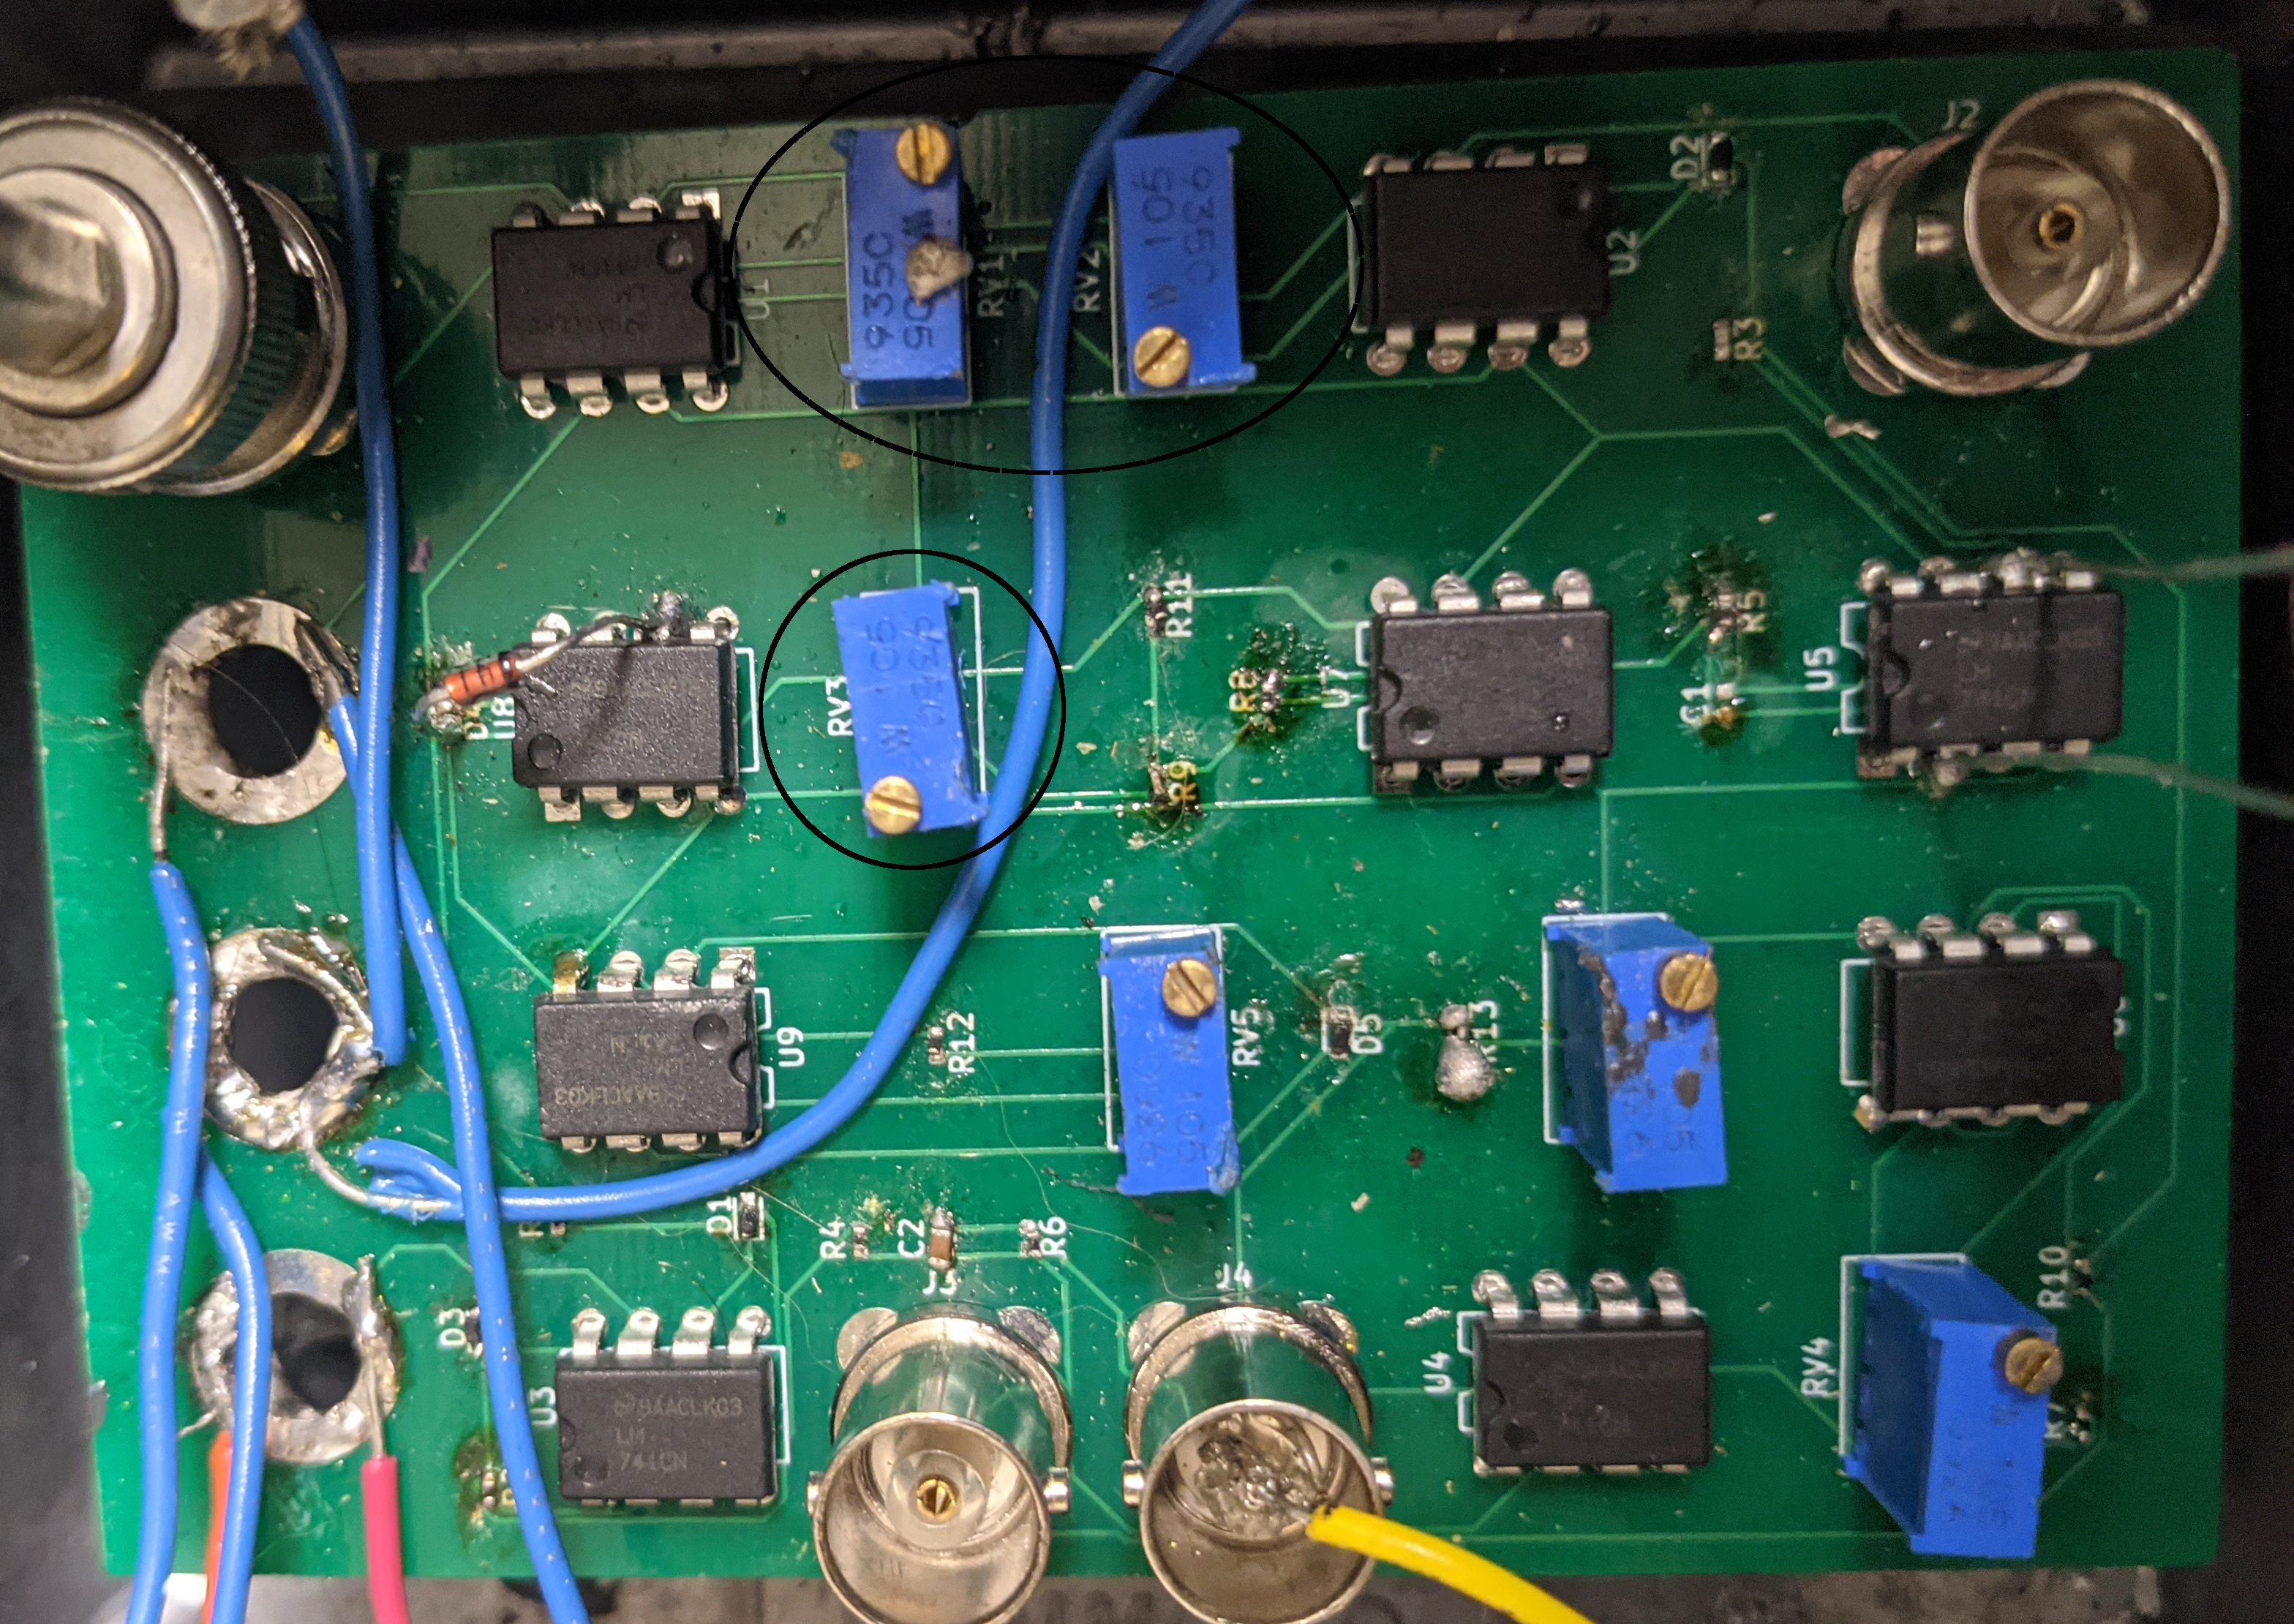
\includegraphics[width=0.7\textwidth]{Data for Probe Writeup/circuit.jpg}
	\caption{Image of circuit from above with trim potentiometers RV1, RV2 and RV3 circled. Potentiometers RV1 and RV2 control the circuit's gain, which should be adjusted to match the FOV-voltage relationship of the particular probe. RV3 controls the output signal's DC offset, which should be adjusted so that the zero points of the input and output match (so that the center of the B-Scan is the A- and M-Scan measurement location).}
\end{figure}

\section{Control programs for fixed background}\label{controlprograms}
\hypertarget{controlprograms}{}

\par{The control programs have been varied from what was discussed in the \href{https://github.com/Brian-Frost-LaPlante/LabReports/blob/main/ProbeReports/Fixed-BackgroundProcessing.pdf}{Fixed-Background Processing report}. I will quickly describe the operation of all of the functions again, focusing mostly on changes made since the last report.}

\par{Fig. \ref{termstart} shows the terminal at the startup of the OCT with Processing program, used for all data acquisition. There are three functions available for the fixed-background processing: \texttt{M: Measure Fixed Background}, \texttt{P: Centered M-Scan with Fixed Background} and \texttt{B: B-Scans with Fixed Background}. I will walk through these functions quickly.}

\begin{figure}[!h]\label{termstart}
	\centering
	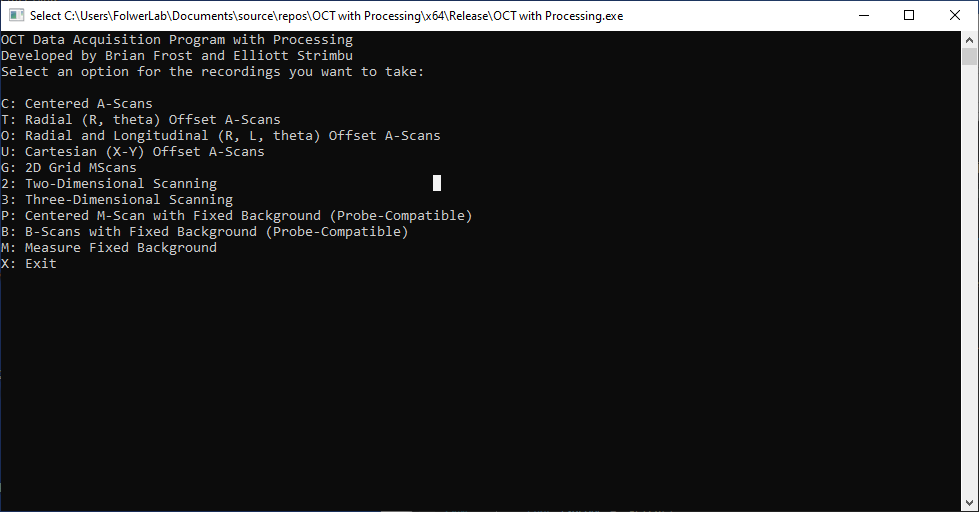
\includegraphics[width=0.6\textwidth]{Data for Probe Writeup/Terminal at Startup.png}
	\caption{Terminal at the start of the OCT with Processing program, with probe-compatible options \texttt{M}, \texttt{P} and \texttt{B}.}
\end{figure}

\subsection{Option M: Measure Background}

\par{Option \texttt{M} takes about 300 A-Scans at the center location, and saves the average photodetector pattern (a list of integers in the wavelength domain) as a text file \texttt{spec} in the directory shown in Fig. \ref{specloc}. This spectrum is written over every time this function is called, so as not to bloat the system with many old backgrounds.}

\par{Also present in this folder for those interested are sample backgrounds taken in air, water and scala tympani, as well as one set taken with the Telesto bulk optics. This can be used to see differences between various backgrounds. To see their associated wavenumber or spatial domain forms, the matrix \texttt{L2K} stored in this folder maps wavelength domain to wavenumber domain, and then a Fourier transform can be taken to see the spatial domain signal.}

\begin{figure}[!h]\label{specloc}
	\centering
	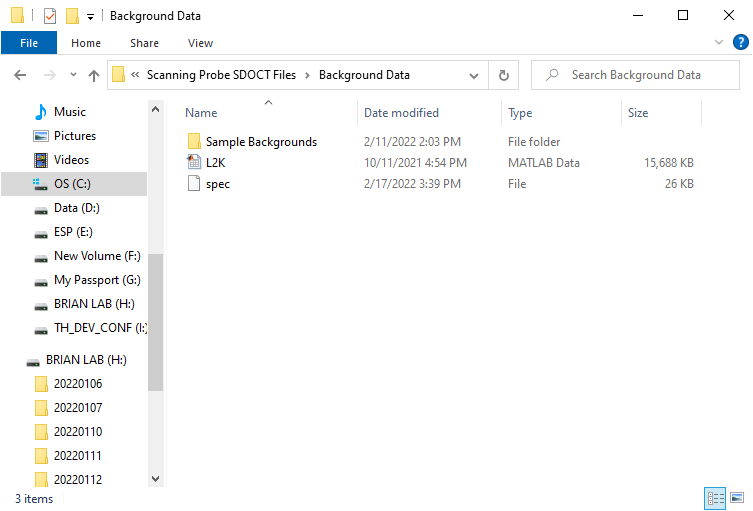
\includegraphics[width=0.6\textwidth]{Data for Probe Writeup/spec location.png}
	\caption{Files related to the measured fixed background, including (1) \texttt{spec}, the last recorded background, (2) \texttt{L2K}, a matrix that maps from the wavelength domain to the wavenumber domain, and (3) a folder full of sample backgrounds taken with the probe and bulk optics in different media.}
\end{figure}

\subsection{Taking and observing B-Scans with fixed background}

\par{Option \texttt{B} has changed significantly since the last report. The program now asks for the field of view to be scanned (in mm), then scans over this FOV with pixel size 0.04 $\mu$m, at 28 kHz sampling rate. The interface is seen in Fig. \ref{optionb}. The B-Scan is then stored in a PNG file called \texttt{BScanUpdate} in the directory shown in Fig. \ref{Bloc}. After this initial acquisition, any time any button other than \texttt{x} is pressed,a B-Scan with the same FOV, pixel size and sampling rate is acquired and stored in the same location, writing over the previous B-Scan.}

\par{A key update to the code is the change in sampling rate. While it had previously been 76 kHz, we discussed in \hyperlink{circsection}{Sec \ref{circsection}} that with the new LPF cutoff frequency, this sampling rate yields a very poor approximation of the ramp at the output of the circuit. Strangely, the ThorLabs SpectralRadar SDK B-Scan function seems to average B-Scans over one second, no matter the sampling rate. For a 10 kHz sampling rate, there are too few samples to average, especially considering that the circuit's transient response. 28 kHz is the best sampling frequency to comprimise between both of these problems.}

\par{The specific line of code that alters the sampling rate is: \texttt{setDevicePreset(Dev, 0, Probe, Proc, 3)}. The first input is the device handle, the second is the index of the parameter you want to set (index 0 is the sampling rate), the third is the probe handle, and the fourth is the index of the value you want to set the parameter to. Here, 0 corresponds to whatever the default is (76 kHz for now), 1 corresponds to 146 kHz, 2 corresponds to 76 kHz, 3 corresponds to 28 kHz (as set here) and 4 corresponds to 10 kHz. I suggest 0 is never used, as the default can be changed in configuration files.}

\par{At any point, the MATLAB script ShowProbeBScan can be called, which asks for the FOV you used to measure the B-Scan in the control program. It also lets you save the B-Scan, in the working directory as both a \texttt{fig} and \texttt{mat} file. While the control program writes over the \texttt{BScanUpdate} file, this allows you to maintain a specific B-Scan for your experiment. The interface for this script can be seen in Fig. \ref{showprobebscan}.}

\par{The script displays the B-Scan with the correct aspect ratio and axis labels as shown in Fig. \ref{bex}. It also shows a red line where the center location (or A-Scan location) is. This figure is updated every time \texttt{ENTER} is pressed in the MATLAB command line, and stops when \texttt{0} is pressed.}

\begin{figure}[!h]\label{optionb}
	\centering
	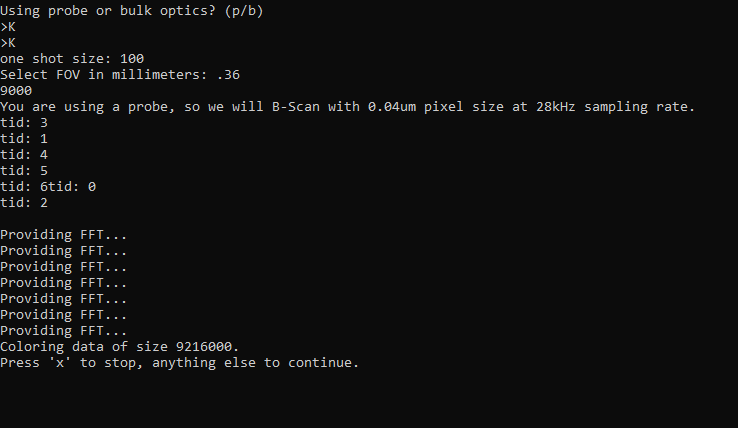
\includegraphics[width=0.6\textwidth]{Data for Probe Writeup/BMode Probe.png}
	\caption{Interface for option \texttt{B} in the OCT with Processing program, which asks for the FOV and then takes scans whenever a button other than \texttt{x} is pressed.}
\end{figure}

\begin{figure}[!h]\label{Bloc}
	\centering
	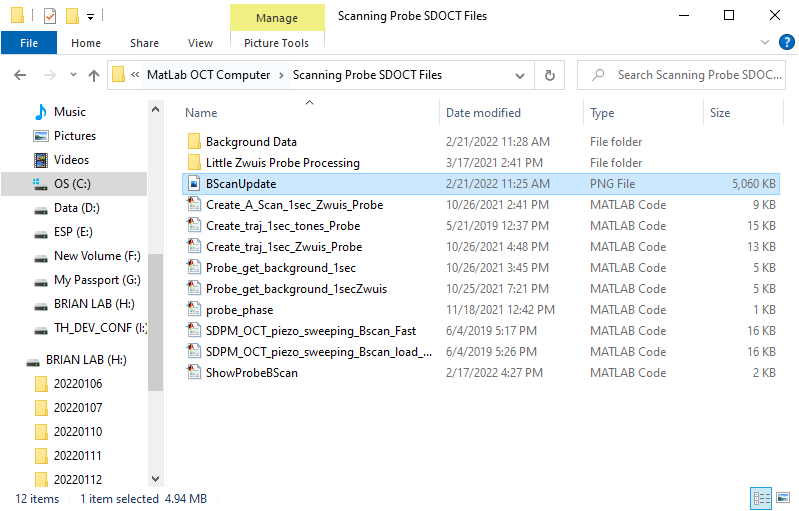
\includegraphics[width=0.6\textwidth]{Data for Probe Writeup/BScan location.png}
	\caption{Location of the B-Scan file saved by the OCT with Processing program's Option \texttt{B}.}
\end{figure}

\begin{figure}[!h]\label{showprobebscan}
	\centering
	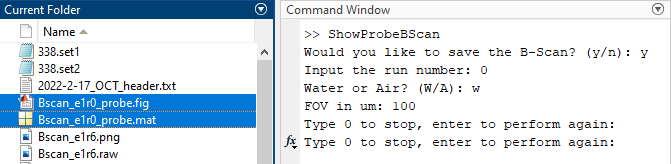
\includegraphics[width=0.6\textwidth]{Data for Probe Writeup/ShowProbeBScan operation.png}
	\caption{Interface of the \texttt{ShowProbeBScan} MATLAB script, with the saved B-Scans highlighted in the working directory. Note that the B-Scan can be updated by pressing \texttt{ENTER} at any time.}
\end{figure}

\begin{figure}[!h]\label{bex}
	\centering
	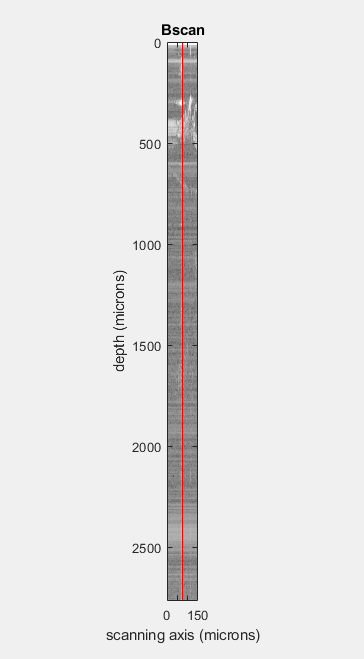
\includegraphics[width=0.6\textwidth]{Data for Probe Writeup/BScan fig update.png}
	\caption{A sample B-Scan generated by the \texttt{ShowProbeBScan} MATLAB script, from an \textit{ex vivo} guinea pig cochlea, FOV 150 $\mu$m. The red line is the center A-Scan in the B-Scan where measurements will be taken.}
\end{figure}

\par{The suggested use for this program is as a replacement for ThorImages B-Scan acquisition. The user can initiate the B-mode control program, take a scan, and then initiate the MATLAB script. Then they can continue to update the B-Scan first in the control program, then in the MATLAB program, by pressing \texttt{ENTER} in the respective command lines. While this is a bit clunkier than ThorImage, it accounts for the background and works nearly in real-time. ThorImage B-Scans which use an incorrect background are low-quality and potentially misleading.}

\subsection{Option P: M-Scans with fixed background}

\par{This method has not been changed at all since the last report. It takes M-Scans without flying back, loads in the \texttt{spec} file last measured with option \texttt{M} and uses it to process the data. The data files created by this program are of the same form as those created by the standard M-Scan programs, and the same analysis MATLAB scripts can be used for these files.}

\section{Using ThorImage with the probe}\label{thorimagesection}
\hypertarget{thorimagesection}{}

\par{When ThorImage takes a B-Scan, it always flies back and takes background shots to use in processing the next B-Scan. Unlike in our control programs, this cannot be turned off in the ThorImage GUI. As a result, when using the probe, ThorImage takes a number of shots while the probe is resetting to its initial position and uses this as the background. That is, the background used by ThorImage while using the probe is an average of the \textit{signal}. This makes for a very distorted B-Scan, but it can still be used as an imperfect guide.}

\par{If this is desired, the settings shown in Fig. \ref{tisettings} should be used. These are the same that are used in our control programs, which perform the same operation while accounting for the fixed background.}


\begin{figure}[!h]\label{tisettings}
	\centering
	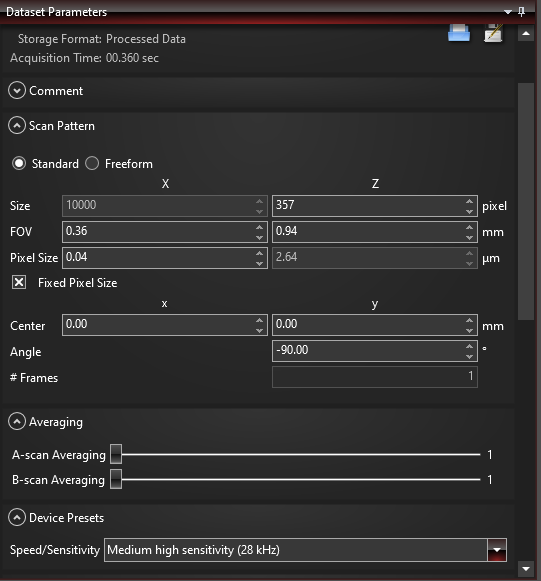
\includegraphics[width=0.6\textwidth]{Data for Probe Writeup/ThorImage settings for BScan.png}
	\caption{B-mode settings in ThorImage for use with the probe.}
\end{figure}


\subsection{The ThorImage ``fake background" trick for A-Scans}

\par{While B-Scans in ThorImage never properly account for the background when using the probe, there is a way that one can force ThorImage to use a proper background while in A-mode. This ``fake background trick" relies on the method by which ThorImage determines the background it uses in A-mode.}

\par{As stated above, ThorImage takes background shots before every B-Scan. However, it does not take backgrounds at all in A-mode. Instead, the A-scan processing in ThorImage is performed using the last background recording taken in B-mode. We can thereby manipulate the background being used in ThorImage A-mode by taking first a B-Scan far from any sample. This records a background while the probe is effectively imaging nothing, equivalent to our \texttt{M: Measure background} control program. Then, we switch to A-Mode. This background, which was the signal from the probe taken far from a sample, will then be used to take A-Scans! This trick can be useful in experiments to see real-time updates of the A-Scan where we will measure our data.}

\section{Signal quality}

\par{In this section, I will discuss results from two important experiments performed with the probe. The first, in which we tested the probe's ability to measure displacement of a piezo shaker in air and water, shows the medium-dependance of the probe's SNR. The second shows an interesting phenomenon related to B-Scans. In both subsections below, I describe the implications these results have on interpreting probe data, and propose a future probe modification.}

\subsection{SNR in air vs. water}\label{SNRsection}
\hypertarget{SNRsection}{}

\par{In this experiment, we used probe D6 to measure the vibration of a piezo shaker driven by a 1V amplitude 15-frequency tone complex both in air and water. We compare this to the vibration measured with the Telesto bulk optics in air. The magnitude responses of the measured displacements are shown in Fig. \ref{airwater}.}

\begin{figure}[!h]\label{airwater}
	\centering
	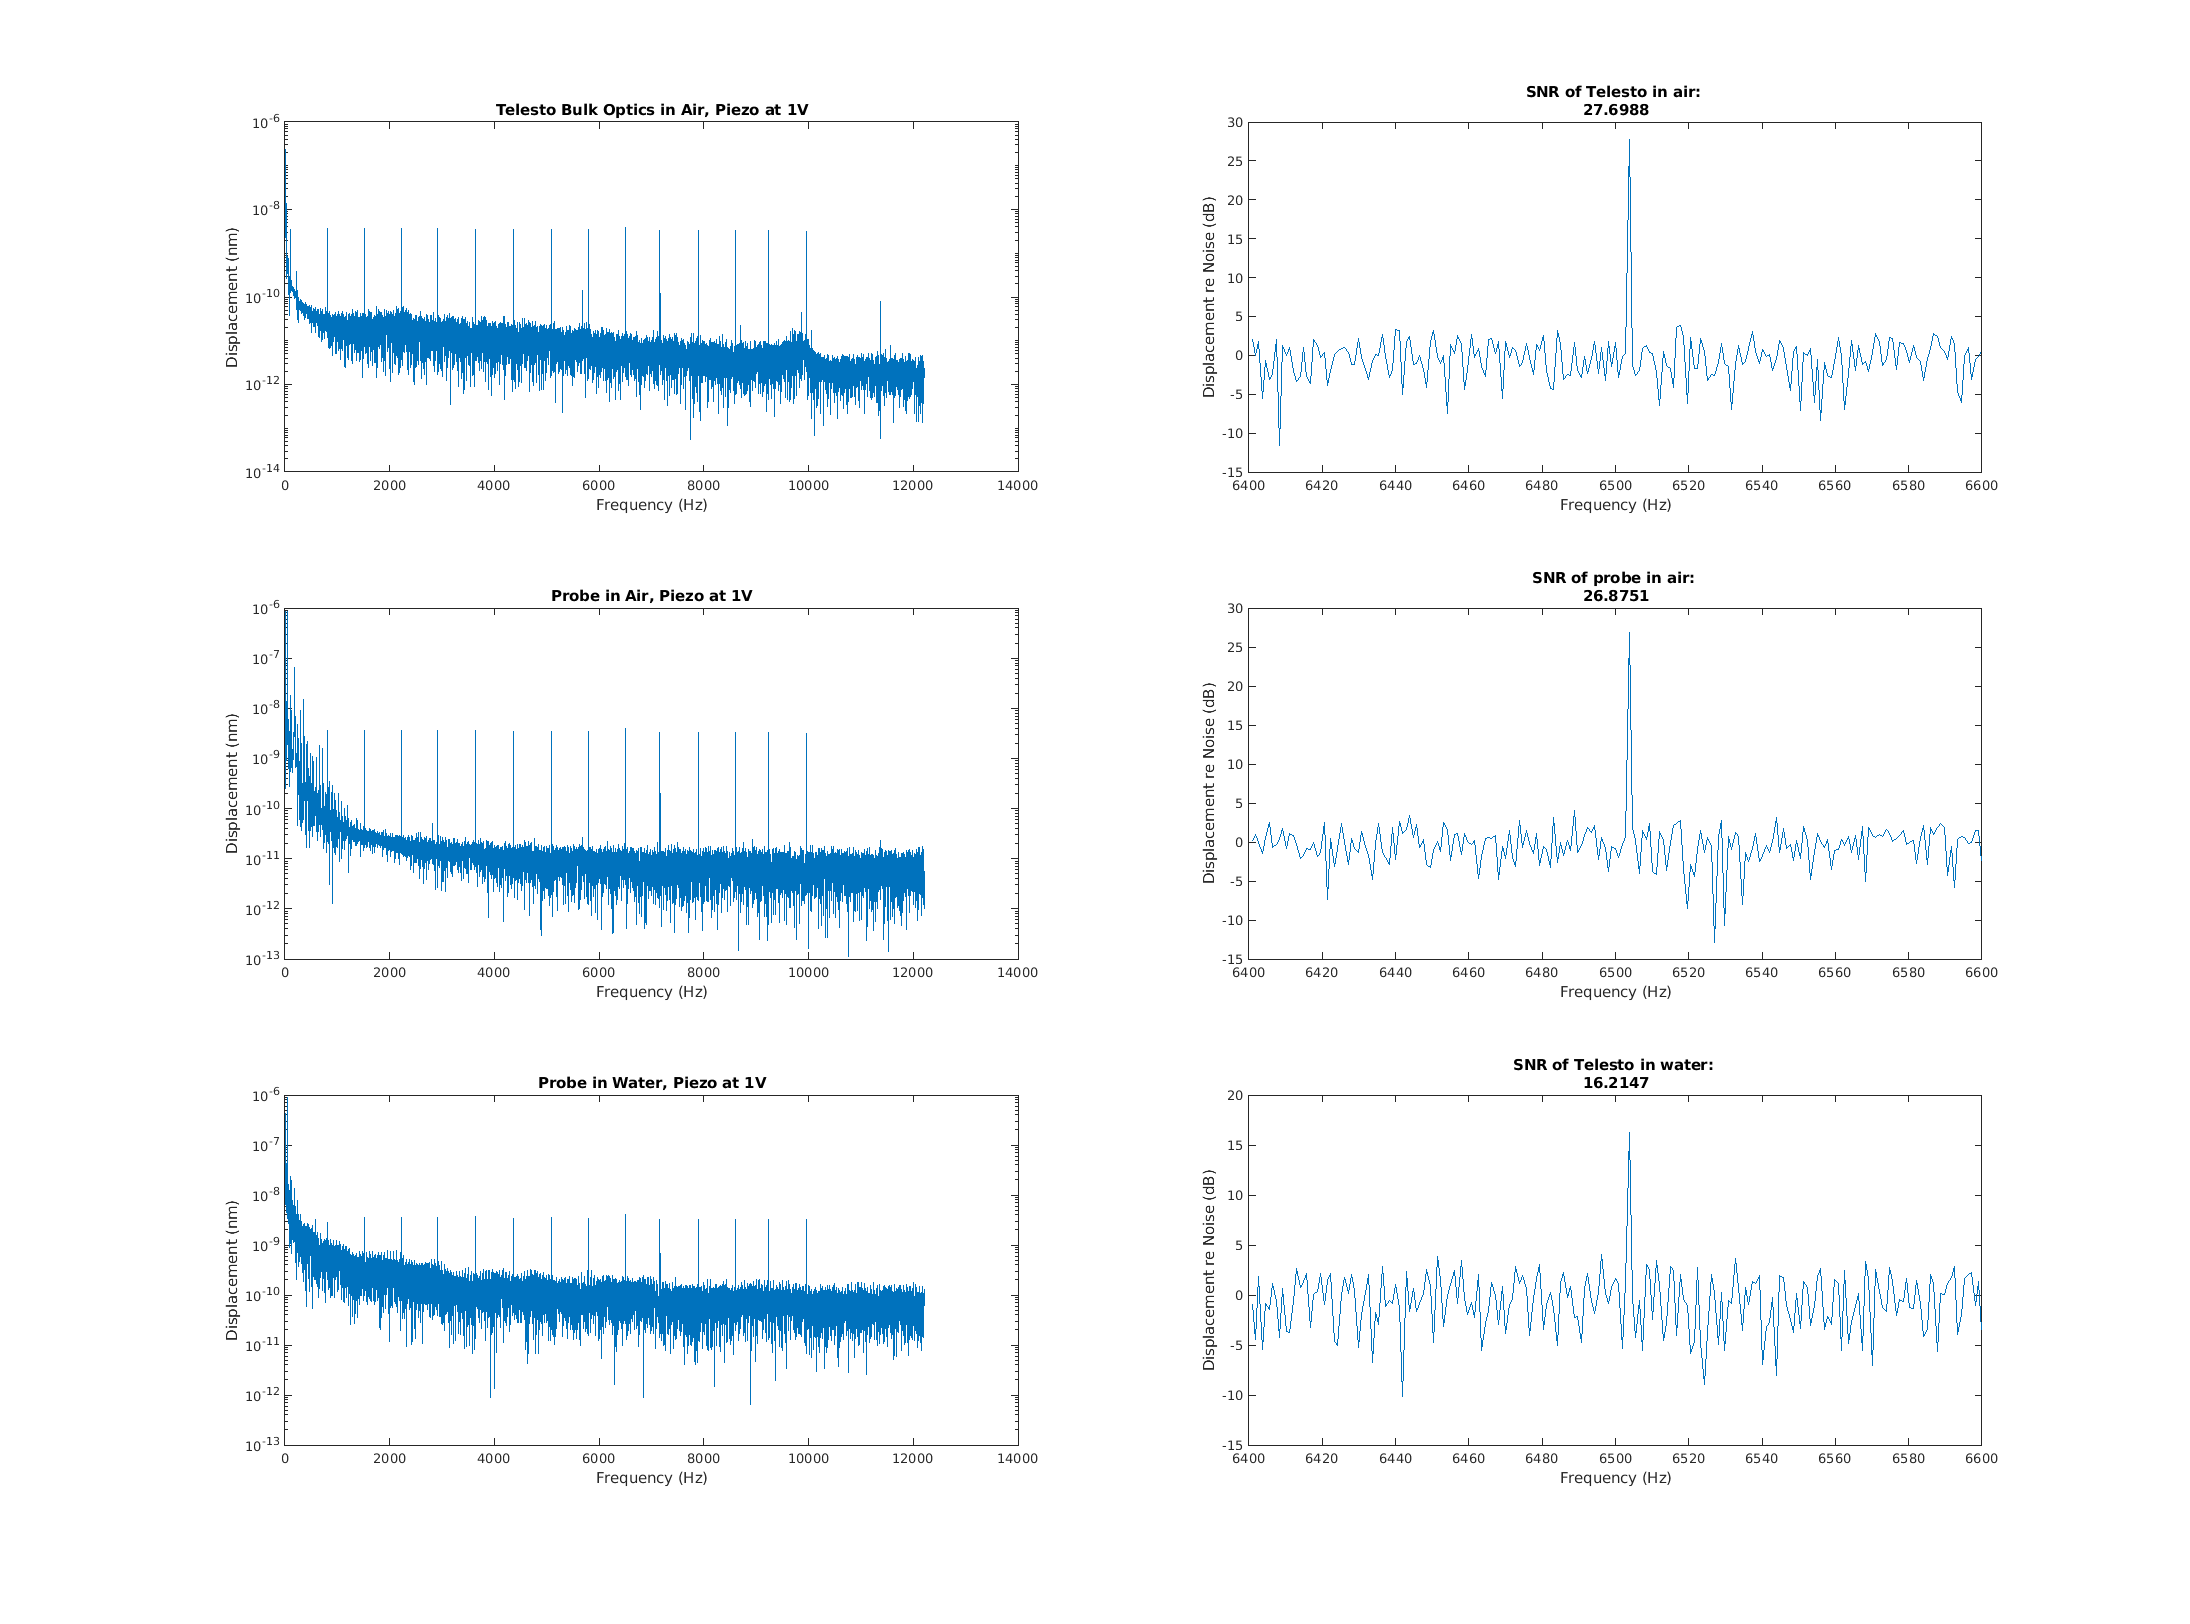
\includegraphics[width=\textwidth]{Data for Probe Writeup/SNRcomp.png}
	\caption{Piezo shaker vibrations in response to 1V amplitude 15-frequency stimulus, measured using Telesto bulk optics in air, probe D6 in air and probe D6 in water. Right-hand subplots show zoomed in magnitude responses re noise level (determined by average surrounding the peak at 6500 Hz) used to determine the SNRs listed in the titles.}
\end{figure}

\par{First we should note that in all cases the method has accurately measured the same displacement magnitude, which is promising. Next, we consider the peak at 6500 Hz to test the SNR. Using the average displacement measured near the peak as the noise level, we can plot the displacement re noise in decibels, shown in the right-hand subplots in Fig. \ref{airwater}. The peak value re noise gives the SNR in dB. The Telesto and probe in air give comparable SNRs of 27.7 dB and 26.9 dB repectively. On the other hand, the probe in water performs significantly worse, with an SNR of 16.2 dB -- 10 dB worse than in air.}

\par{In \hyperlink{bgsection}{Sec. \ref{bgsection}}, we describe how the probe's reference beam intensity is determined by what is reflected at the tip of the probe. This is entirely controlled by the index of refraction of the medium vs. the glass. The index of air is about 1, that of water is about 1.3 and that of glass is around 1.4. This means that the probe is ``better matched" to water than air, so less light is reflected at the tip in water. This decrease in reference intensity seems to be having a negative effect on the SNR. This will affect both imaging and vibrometry SNR.}

\par{As the probe's reference beam intensity is determined only by the index of the tip, we must turn to a mechanical solution to this problem. One suggested method (in the works) is to apply a think gold film to the tip of the probe of a thickness determined so as to have a esirable amount of reflecatance at the tip, ideally more similar to what is achieved in air.}

\subsection{B-Scan quality}\label{BScansection}
\hypertarget{BScansection}{}

\par{When we first started taking measurements using the probe in the cochlea, \textit{in} and \textit{ex vivo}, we noticed that the average A-Scans from each M-Scan often had very poor SNR. However, we were perplexed by the fact that B-Scans often looked quite nice, using the same background processing.}

\par{For example, see Fig. \ref{bvsa}, taken in an \textit{ex vivo} guinea pig cochlea. The leftmost panel is a B-Scan containing the organ of Corti, the center panel is the central A-Scan of that B-Scan, and the right-most panel is the averaged A-Scan at the center from a one-second M-Scan.}

\begin{figure}[!h]\label{bvsa}
	\centering
	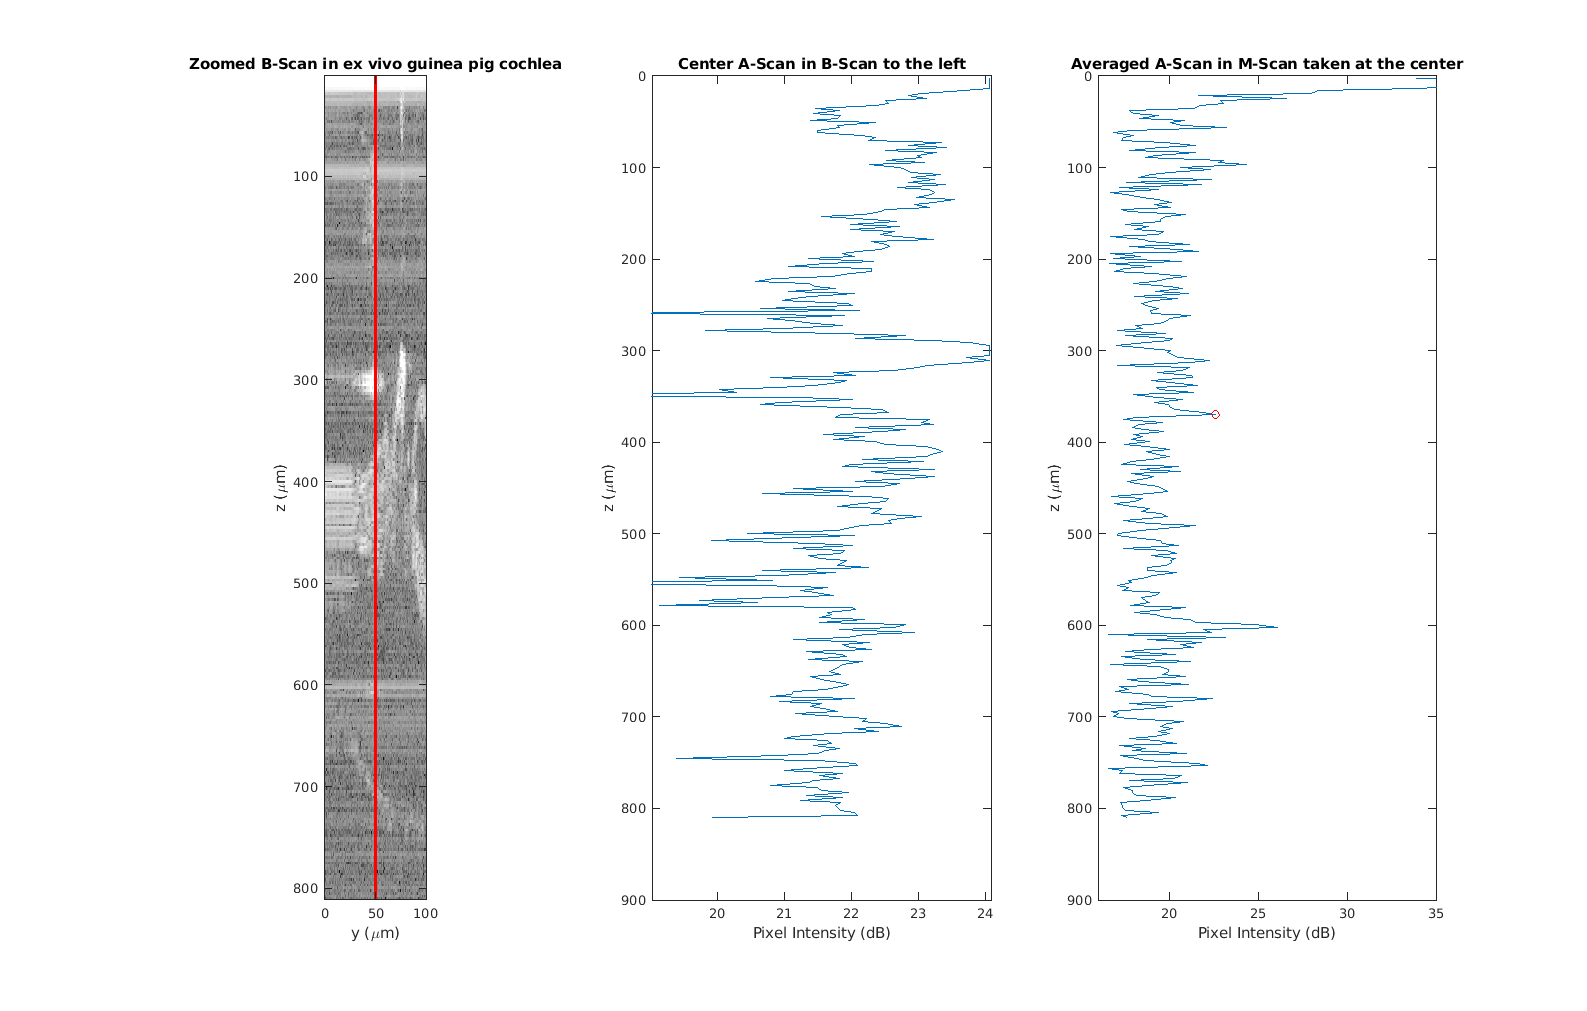
\includegraphics[width=\textwidth]{Data for Probe Writeup/Data 2022-2-17/BScan v AScan.png}
	\caption{Left to right: A B-Scan, the center A-Scan in that B-Scan and the averaged A-Scan from an M-Scan taken at the center. A red dot indicates the point in the averaged A-Scan where the B-Scan indicates that the basilar membrane is located, about 3 dB out of the noise. In the central A-Scan of the B-Scan (middle panel), this peak is present but in the noise. Note that the SNR for all pixels corresponding to structures is never more than 1.5 dB in the central A-Scan, while some structural peaks are about 3 dB out of the noise in the M-Scan average. Neither are high-quality.}
\end{figure}

\par{In the B-Scan, structures can be made out by eye -- it is clear where the orgam of Corti is relative to fluid spaces of Scala Tympani and Scala Media. However, both the center A-Scan and the averaged A-Scan have very low SNR. Of particular interest is that the center A-Scan from this B-Scan has less than 2 dB SNR despite the image looking ``pretty good."}

\par{The phenomenon at play here is that while no individual column in the B-Scan has high SNR, our eyes visually average nearby pixels in 2D, allowing us to see a shape well, even though it is not very far out of the noise. This is analogous to the impressionist technique of pointillism employed by artists such as van Gogh and Seurat, wherein from afar our eyes will mix nearby colors automatically. Fig. \ref{seurat} illustrates this concept, where the ``pixels" are small dots of paint which look like ``noise" until we are sufficiently zoomed out so that the colors are mixed by our eyes.}

\begin{figure}[h!]\label{seurat}
	\centering
	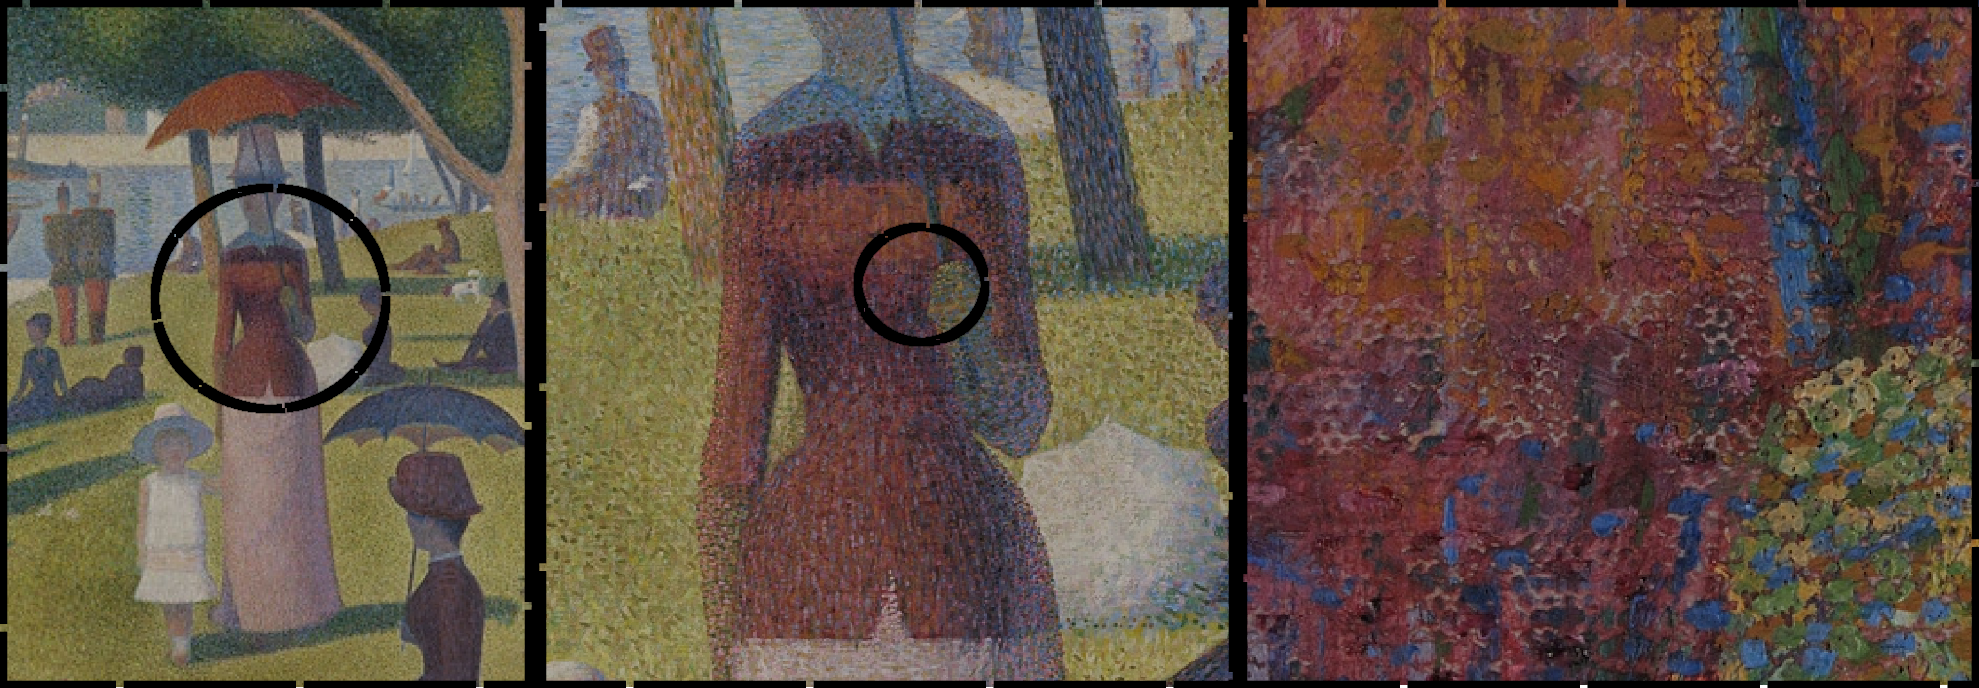
\includegraphics[width=\textwidth]{Data for Probe Writeup/seurat.png}
	\caption{.}
\end{figure}

\par{I suggest making use of this optical phenomenon: we can use the B-Scan to locate pixel positions of anatomical structures, then pick those pixels in the averaged A-Scan to measure from even if they are not far out of the noise. This allows us to use averaged spatial information in 2D and the power of the human mind to determine structure locations in low-quality 1D scans.}

\par{We should note, finally, that these data are all from a cochlea of a dead animal, which degrades the signal quality. They were also taken in water, which we know leads to poor SNR from the previous subsection.}

\end{document}
